\documentclass[12pt]{article}
\usepackage[left=1.2in,right=1in]{geometry}
\usepackage{graphicx}
\usepackage{fancyhdr}
\usepackage{lastpage}
\pagestyle{fancy}
\lhead{Chen CC}
\chead{Homework}
\rhead{\thepage\ of \pageref{LastPage}}


\begin{document}
\title{The Dissipative Particle Dynamic Simulation of Suspension in Micro-channels}
\author{Chen CC, Zhou WW\footnote{Corresponding author}}
\maketitle

\begin{abstract}
This paper investigated the transport and conformation of macromolecules in microchannels using the dissipative particle DPD and finite extensible nonlinear FENE based spring chains model. This paper investigated the transport and conformation of macromolecules in microchannels using the dissipative particle DPD and finite extensible nonlinear FENE based spring chains model.  This paper investigated the transport and conformation of macromolecules in microchannels using the dissipative particle DPD and finite extensible nonlinear FENE based spring chains model.  
\end{abstract}

\section{Introduction}
This paper investigated the transport and conformation of macromolecules in microchannels using the dissipative particle DPD and finite extensible nonlinear FENE based spring chains model.  This paper investigated the transport and conformation of macromolecules in microchannels using the dissipative particle DPD\cite{Chun1999Fabrication,Fan2003Microchannel}.  

This paper investigated the transport and conformation of macromolecules in microchannels using the dissipative particle DPD.  

This paper investigated the transport and conformation of macromolecules in microchannels using the dissipative particle DPD.  DPD and finite extensible nonlinear FENE based spring chains model. This paper investigated the transport and conformation of macromolecules in microchannels using the dissipative particle DPD.

\section{Methodology of the dissipative particle dynamics}
This paper investigated the transport and conformation of macromolecules in microchannels using the dissipative particle DPD and finite extensible nonlinear FENE based spring chains model.  This paper investigated the transport and conformation.
\begin{equation}
\frac{\mathrm{d}r_i}{\mathrm{d}t}=v_i,\qquad
\frac{\mathrm{d}v_i}{\mathrm{d}t}=\sum_{j \neq i}^N {f_{{ij}_i}^{ext}}
\end{equation}
Where $r_i$ and $v_i$ denote the position and velocity of particle $i$.

\begin{equation}
\mathrm{F}_{ij}^C=
\left\{\begin{array}{ll}
a_{ij}(1-r_{ij})&r_{ij}<r_C\\
0&r_{ij}\geq r_C
\end{array}\right.
\end{equation}

\section{Parameters}
To construct a working DPD, we need select values of some necessary parameters. To construct a working DPD, we need select values of some necessary parameters. Table \ref{tab:mopa}  listed the some model parameters that we need determined before we could sufficient.
\begin{table}[htb]
\centering
\caption{Model parameters}\label{tab:mopa}
\begin{tabular}{|l|c|c|}
\hline
\textbf{Model parameters}&\textbf{Symbol}&\textbf{Value}\\
\hline
Mass of DPD paticle&m&unity\\
\hline
Simulation time step& t&unity\\
\hline
\end{tabular}
\end{table}

\section{Channel flow of FENE chain suspension}
We use DPD particles and FENE chains to model the suspension of macromolecules in three kind of micro-channels. We use DPD particles and FENE chains to model the suspension of macromolecules in three kind of micro-channels, which are shown in figure \ref{fig:quad} and figure \ref{fig:slop} respectively.

We use DPD particles and FENE chains to model the suspension of macromolecules in three kind of micro-channels. \par
We use DPD particles and FENE chains to model the suspension of macromolecules in three kind of micro-channels. FENE chains to model the suspension of macromolecules in three kind of micro-channels. 

\begin{figure}[htb]
\begin{minipage}[t]{0.48\textwidth}
\centering
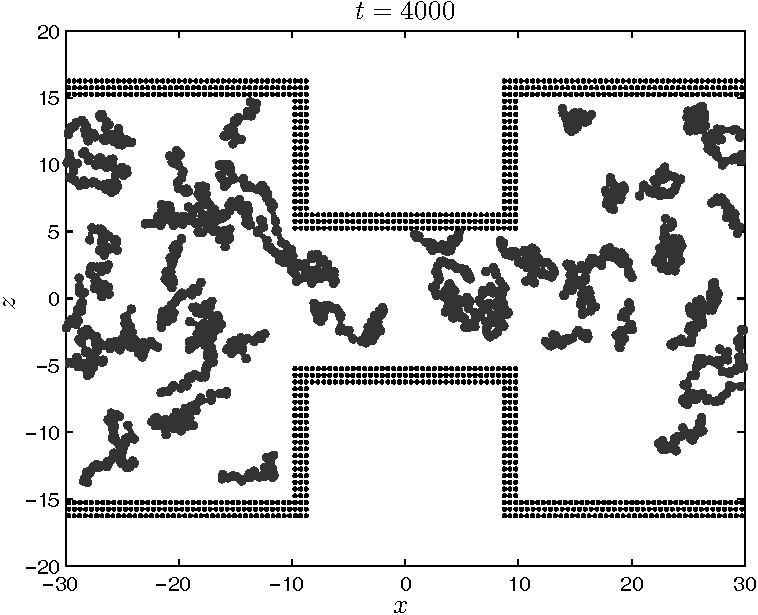
\includegraphics[width=0.95\textwidth]{chainT4000s}
\caption{Quadrate contraction micro}\label{fig:quad}
\end{minipage}
\begin{minipage}[t]{0.48\textwidth}
\centering
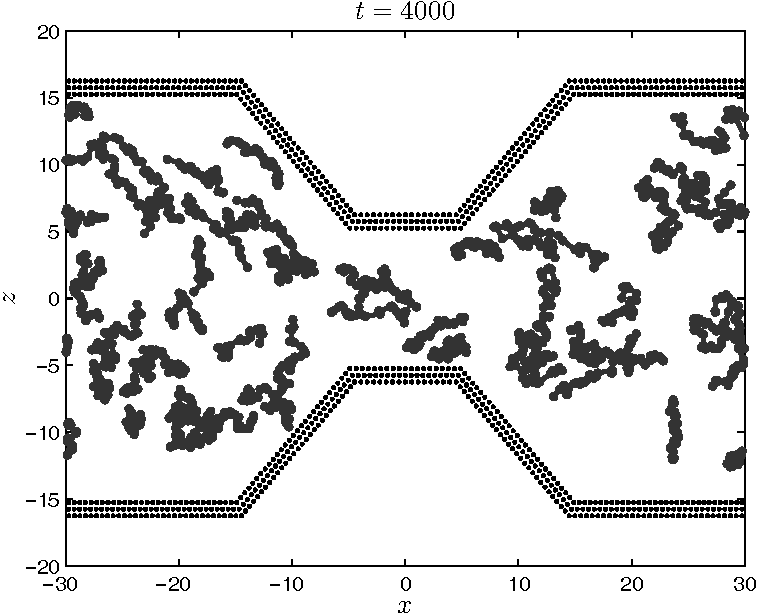
\includegraphics[width=0.95\textwidth]{chainY4000s}
\caption{Sloping contraction micro}\label{fig:slop}
\end{minipage}
\end{figure}

\section{Conclusion}
Our numerical results show that macro are mainly concentrated in the middle channel. We use DPD particles and FENE chains to model the suspension of macromolecules in three kind of micro-channels. 

We use DPD particles and FENE chains to model the suspension of macromolecules in three kind of micro-channels. 

Our numerical results show that macro are mainly concentrated in the middle channel. We use DPD particles and FENE chains to model the suspension of macromolecules in three kind of micro-channels. 


\bibliographystyle{unsrt}
\bibliography{cc}

\end{document}